\documentclass{article}
\usepackage[utf8]{inputenc}
\usepackage{blindtext, graphicx}
\begin{document}

\section{ Assignment 1 Question 4}
($p_{1x}$,$p_{1y}$);($p_{2x}$,$p_{2y}$);($p_{3x}$,$p_{3y}$) and similarly for Iq are in the camera pixel coordinate system. So let us find the direction of the vanishing points by using the focal length and the resolution of both the camera. Assuming ($c_{1x}$,$c_{1y}$) and ($c_{2x}$,$c_{2y}$) as the origin of the image coordinate system i.e the optical center.
The image coordinates are in the Z = fp and Z=fq plane respectively.
So the direction of $P_1$,$P_2$,$P_3$ will be the coordinate of there vanishing point subtracted from the optical center and muktiplied by the resolution. Hence :-

$P_1$ = ($s_p$($p_{1x}$-$c_{1x}$),$s_p$($p_{1y}$-$c_{1y}$),$f_p$).
 $P_2$ = ($s_p$($p_{2x}$-$c_{1x}$),$s_p$($p_{2y}$-$c_{1y}$),$f_p$).\\
  $P_3$ = ($s_p$($p_{3x}$-$c_{1x}$),$s_p$($p_{3y}$-$c_{1y}$),$f_p$).
  
   $Q_1$ = ($s_q$($q_{1x}$-$c_{2x}$),$s_q$($q_{1y}$-$c_{2y}$),$f_q$).
 $Q_2$ = ($s_q$($q_{2x}$-$c_{2x}$),$s_q$($q_{2y}$-$c_{2y}$),$f_q$).\\
  $Q_3$ = ($s_q$($q_{3x}$-$c_{2x}$),$s_q$($q_{3y}$-$c_{2y}$),$f_q$).
  
 Now these directions of P and Q will be related to each other in teh same way as the camera orientation. That is \textbf{R}[P1 P2 P3] = [Q1 Q2 Q3].From this equation we get the \textbf{R} matrix. 
 
 Now directions are only connected by rotation or orientation. Translation can't effect the direction of a line. Hence i guess it wont be possible to determine the translation matrix untill we are given some other relation between the vanishing points.

Now as the 3 directions are mutually perpendicular, there dot product should be zero. this will give us one equation. 
   $$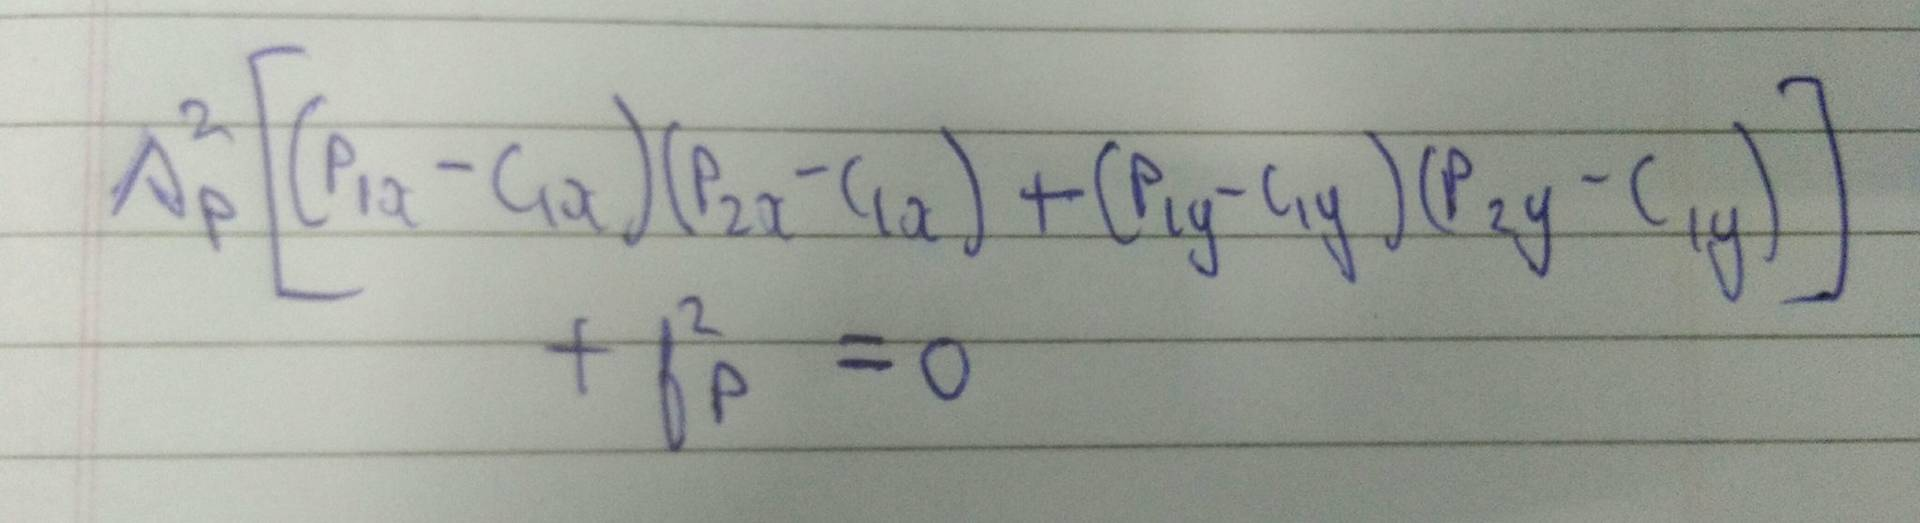
\includegraphics[width=0.8\textwidth]{img.jpg}\\[0cm]
$$
And as per the paper from " Camera calibration using two or three vanishing points Radu Orghidan et.al " the orthocenter of the triangle formed by the 3 vanishing points gives us the optical center of the camera. 
Using this we will be able to get the optical center.
Now from the mutually perpendicular equation, which has both $s_p$ and $f_p$ we can get an equation relating them but not exact value.
\end{document}
